\documentclass{article}

\usepackage{amsmath}
\usepackage{amssymb}
\usepackage{amsfonts}
\usepackage{graphicx}
\usepackage{hyperref}
\usepackage{geometry}
\usepackage{tikz}

\geometry{a4paper, margin=1in}

\title{Visualization of Sound Spectra of a Whistle}
\author{Jorge R. Gherson}

\begin{document}

\maketitle
\newpage 

\tableofcontents
\newpage

\section{General Objective}
We have a dataset containing the sound spectra of a whistle collected at different mass 
flow rates, pressures, and frequencies. The main objective of this project is to 
visualize the sound spectra in a way that would allow a Convolution Neural Network (CNN) 
or a human to efficiently see the relationship between the sound spectra and the 
mass flow rate. 

\section{Exploratory Analysis of the Sound Spectra Dataset}\label{exploratory_analysis}
The initial data analysis was carried out in a Jupyter notebook named \verb|initial_analysis.ipynb|.
First, it is necessary to import the required libraries and load the dataset. The dataset 
was given in a \verb|.mat| file, which was then loaded using the \verb|scipy.io| library. 
We have a dataset that contains 267 measurement instances for the following variables: 
\begin{enumerate}
    \item \(P_\text{all}\): A 2D array containing the sound pressure (in Pascals) 
    for each frequency and time point. 
    \item \verb|amplitude_all|: A 2D array containing the amplitude of the sound for each 
    frequency and time point. 
    \item \verb|frequency_all|: A 2D array containing the Fast Fourier Transform (FFT) 
    frequencies with 49902 points. 
    \item \verb|m_dot_all|: A 2D array containing the mass flow rate (in kg/s) for each 
    frequency and time point.
    \item \verb|signal_all|: A 2D array containing the 1 second worth of the original 
    microphone signal collected at 100,0000 Hz.
\end{enumerate}

First, I sought to understand the structure of the dataset by checking the shapes of 
each variable. The shapes of the variables are as follows:

\begin{verbatim}
    P_all (267, 1)
    amplitude_all (267, 1)
    frequency (49902, 1)
    m_dot_all (267, 1)
    signal_all (267, 1)
\end{verbatim}

Notice all of the lengths agree, except for the frequency variable, which has a different 
shape. This is because the frequency variable contains the FFT frequencies, which are 
the same for all samples, while other variables contain data for each sample. Then, I 
evaluated if the 267 amplitudes correspond with every \(N\)th frequency, where \(N\) is 
the number of frequencies. Finding the ratio between data points in the frequency 
variable and the amplitude variable gave us a ratio of 186. This means that the 
amplitude variable is not evenly distributed across the frequencies, which is an 
important observation for the visualization process.  

Then, I proceeded to unpack each variable and asign it to a respective one in Python 
to evaluate how the data was structured, finding that data stored in the \verb|.mat| file 
is passed as a dictionary in Python (Note: not sure.). Running for \verb|amplitude_all|
yielded: 

\begin{verbatim}
    array([[array([[8.72111064e-05],
               [3.07487090e-04],
               [2.17788468e-04],
               ...,
               [4.34430331e-06],
               [4.19685731e-06],
               [1.59920000e-06]], shape=(49902, 1))],
       [array([[3.06550360e-04],
               [6.16053321e-04],
               [2.33531321e-04],
               ...,
               [3.32547277e-06],
               [1.64016323e-06],
               [9.15600000e-07]], shape=(49902, 1))],
       [array([[1.70402252e-04],
               [1.92546836e-04],
               [2.33929164e-04],
               ...,
               [2.84986090e-06],
               [2.47268173e-06],
               [1.11950000e-06]], shape=(49902, 1))],
       [array([[3.62037875e-04],
               [3.37830354e-04],
               [1.09858487e-03],
               ...,
...
               [9.88551412e-04],
               ...,
               [3.28158474e-05],
               [3.24278557e-05],
               [3.83440000e-06]], shape=(49902, 1))]], dtype=object)
\end{verbatim}

Running so for \verb|signal_all| yielded similar results. Notice that both objects 
have a shape (49902, 1), so it makes sense to make the spectrum 1D and adding them 
vertically. For the amplitudes: 

\begin{verbatim}
        amplitude_all = np.vstack([
                amplitude_all[i].flatten()
                for i in range(len(amplitude_all))
        ])
\end{verbatim}

And for the frequecies: 

\begin{verbatim}
        signal_all = np.vstack([
                sig.flatten()
                for sig in signal_all
        ])
\end{verbatim}

Which yielded: 

\begin{verbatim}
        Amplitude Shape: (267, 49902)
        Amplitude Dimension: 2
        Amplitude dtype: float64
\end{verbatim}
and 
\begin{verbatim}
        Signal Shape: (267, 100000)
        Signal Dimension: 2
        Signal Data Type: float64 
\end{verbatim}

Now it is necessary to note that, for frequency analysis it is 
convenient to implement a logarithmic scale, whhich was calculated using: 

\begin{equation}
        \log(\nu) = 20\log{(A + 1\times 10^{-12})}
\end{equation}

where \(\nu\) represents the frequency and \(A\) the amplitude. We also add \(1\times 10^{-12}\)
to take noise into account. These were then normalized using 

\begin{equation}
        \nu_\text{norm} = \log{\nu} - \max{\log{\nu}}.
\end{equation}

Then, peak frequencies were extracted by implementing masking to crop the data. 
In order to visualize the relationsip, we must sort the mass flow rates and frequencies. 
Then, I defined a sampling rate of \(48000\) Hz, which I used as a parameter for 
the Fast Fourier Transform (FFT) applied using Welch's method. Then, I converted the 
power to decibels (dB) using a logarithmic scale, and I normalized them relative to the maximum. 
These were afterwards sorted, and plotted using a heatmap that yielded:  

\begin{center}
        \begin{figure}
        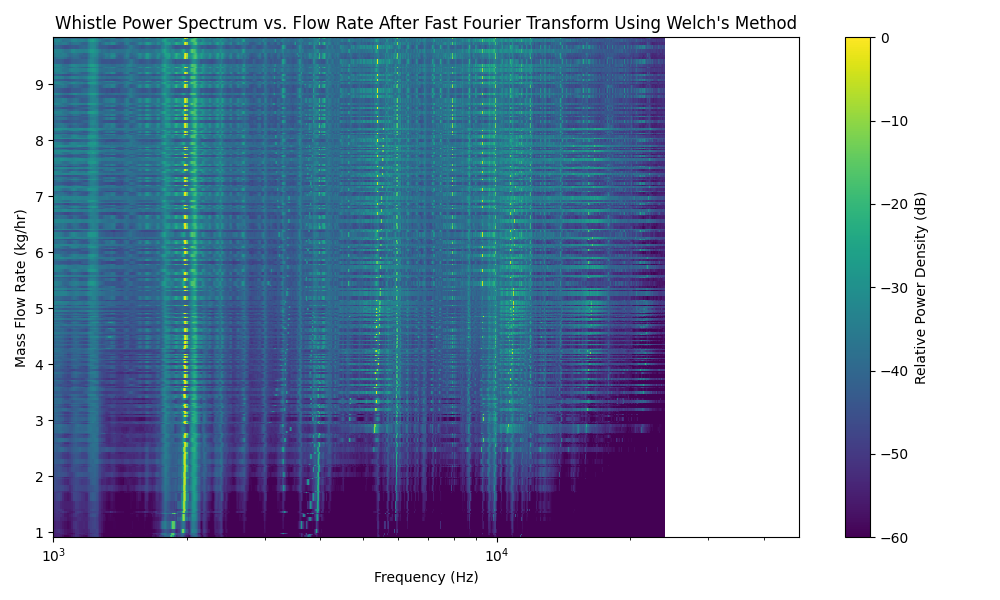
\includegraphics[scale=0.7]{images/spectrum_flowrate_afterFFT.png}
        \caption{The spectrum plotted against the mass flow rate in a logarithmic scale 
        after having applying Welch's method for FFTs.}
        \end{figure}
\end{center}

Notice for this graph that, if the oscillations 

\newpage

\section{Mathematical Formulation}
In order to make the relationship easily visible for a Convolution 
Neural Network, I will carry out a mathematical definition for how 
the network transforms the raw acoustic spectrum into a mass flow rate prediction. 

Let our normalized acoustic spectrum for a single flow rate be 
defined as a one-dimensional vector 

\begin{equation}
        \mathbf{x} = \begin{bmatrix}
                x_1 & x_2 & \cdots & x_N
        \end{bmatrix}^T
\end{equation}

where \(N\) is the total number of frequency bins. The core operation of 
a CNN is the discrete 1D convolution, which applies a set of \(K\) 
trainable kernels (i.e., filters) to the input to detect features like 
whistle peaks or harmonic intervals. 

Let a single filter be a vector \(\mathbf{w}^{(k)}\) of length \(M\). 
The convolution operation computes a new sequence \(\mathbf{z}^{(k)}\) 
for this filter. The \(i\)-th position is given by: 

\begin{equation}
        z_i^{(k)} = \sum_{j=1}^{M} \mathbf{x}_{i+j-1}\cdot \mathbf{w}_j^{(k)} + b^{(k)}
\end{equation}

where \(\mathbf{w}_j^{(k)}\) represents the weights of the \(k\)-th filter, and
\(b^{(k)}\) the bias of the \(k\)-th filter. This represents a mathematical 
cross-correlation. When the shape of the filter matches the shape of a peak 
in the spectrum, \(z_i\) spikes. To allow the network to learn complex, non-linear physical relationships, 
we apply a Rectified Linear Unit (ReLU) to the output of the convolution: 

\begin{equation}
        h_i^{(k)} = \max{(0, z_i^{(k)})}.
\end{equation}

Then, pooling reduces the size of the data, making the model computationally efficient and ``translation invariant.''
The maximum pooling takes the maximum value over a sliding window of size \(P\): 

\begin{equation}
        p_i^{(k)} = \max{h_{P(j-1)+1}^{(k)}, \cdots, h_{Pj}^{(k)}}.
\end{equation}

Later in the network, we use global average pooling (GAP), which takes the average of the entire remaining sequence 
of length \(L\) for each filter \(k\), resulting in a single scalar value per filter: 

\begin{equation}
        g^{(k)} = \frac{1}{L}\sum_{i=1}^L h_i^{(k)},
\end{equation}

which flattens the matrix into a vector \(\mathbf{g} = \begin{bmatrix} g^{(1)} & g^{(2)} & \cdots & g^{(K)}\end{bmatrix}^T\). 
Once the spatial features (i.e., peaks, harmonics) are extracted and flattened into the vector \(\mathbf{g}\), a standard 
neural network layer combines them to predict the flow rate. Let \(\mathbf{W}_d\) be the weight matrix of the dense layer and 
\(b_d\) be the bias vector of the dense layer. Then, 

\begin{equation}
        \mathbf{d} = \max{(0, W_{d\mathbf{g}}+b_d)}.
\end{equation}

Since we are predicting a continuous physical variable, the final layer is a single node with a linear activation function: 

\begin{equation}
        \hat{y} = \mathbf{w}_{\text{out}}^T d + b_{\text{out}}
\end{equation}

where \(\hat{y}\) represents the predicted mass flow rate \(y\) and \(\mathbf{w}_{\text{out}}\) represents the final weight vector mapping 
the learned features to the prediction. However, in order to train a network efficiently, we must also define how ``wrong'' our predictions can be 
compared to the actual mass flow rate. For regressions, we usually use Mean Squared Error (MSE) over a batch of \(B\) training samples: 

\begin{equation}
        L = \frac{1}{B}\sum_{i=1}^B (\hat{y}_i - y_i)^2
\end{equation}

% \newpage 
% 
\section{Mechanics of Sound}
Sound is a longitudinal wave that propagates through a medium (like air) due to the vibration of particles.
The sound spectrum of a whistle is influenced by several factors, including the geometry of the whistle, the flow rate of the air, and 
the pressure conditions -- as featured in \ref{exploratory_analysis}. The mass flow rate, in particular, 
affects the velocity of the air passing through the whistle, which consequently influences the frequency and amplitude of the 
sound produced. \\

\textbf{Quick Note:} From now on, I will use multivariable calculus to derive how this is a one-dimensional problem. Feel free to skip this 
section if you are not familiar with it. \\

Let \(u(\mathbf{k}\cdot\mathbf{r} -vt, t)\) represent the displacement of the sound wave with wave number \(\mathbf{k}\) at 
position \(\mathbf{r}\) during some time \(t\). The wave equation in three dimensions is given by: 

\begin{equation}\label{wave_equation_3d_simple}
        \nabla^2 u - \frac{1}{c^2}\frac{\partial^2 u}{\partial t^2} = 0.
\end{equation}

For our case, we assume that the sound wave is propagating primarily in one direction (say, along the \(\hat{x}\) axis), which allows us to simplify 
the wave equation to one dimension:

\begin{equation}\label{wave_equation_1d_simple}
        \frac{\partial^2 u}{\partial x^2} - \frac{1}{c^2}\frac{\partial^2 u}{\partial t^2} = 0.
\end{equation}

\newpage

\section{Software Implementation Pipeline}\label{implementation_pipeline}

This section provides a detailed walkthrough of how each Python file in the project implements the data processing, 
model training, and evaluation workflow. The software pipeline is designed to be modular, allowing each component 
to be executed independently or as part of a complete machine learning workflow.

\subsection{Configuration Management (\texttt{config.py})}

The \texttt{config.py} file serves as the central configuration hub for the entire project. It defines all 
hyperparameters, file paths, and signal processing constants in a single location, enabling easy modification 
without editing multiple files.

\subsubsection{Key Components:}
\begin{itemize}
    \item \textbf{File Paths:} Defines \verb|DATA_PATH| (path to the raw \texttt{.mat} file) and \verb|PROCESSED_DIR| 
    (directory for storing processed NumPy arrays).
    \item \textbf{Audio Parameters:} 
    \begin{itemize}
        \item \verb|fs = 48000|: Sampling frequency in Hz
        \item \verb|f_min = 100|: Minimum frequency for extraction (Hz)
        \item \verb|f_max = 20000|: Maximum frequency for extraction (Hz)
        \item \verb|epsilon = 1e-12|: Small constant to prevent $\log(0)$ errors
    \end{itemize}
    \item \textbf{Spectrogram Parameters:} Settings for scipy's spectrogram function (\verb|spec_nperseg|, \verb|spec_noverlap|, \verb|spec_window|)
    \item \textbf{Welch's Method Parameters:} Settings for 1D PSD estimation. 
    \begin{itemize}
        \item \verb|welch_nperseg = 4096| 
        \item \verb|welch_window = 'hann'| 
        \item \verb|welch_vmin_db = -120|
    \end{itemize}
    \item \textbf{STFT Parameters:} Settings for 2D time-frequency representation.
    \begin{itemize}
        \item \verb|stft_nperseg = 512|: Window size for STFT (provides time-frequency tradeoff)
        \item \verb|stft_noverlap = 256|: 50\% window overlap
        \item \verb|stft_window = 'hann'| 
        \item \verb|stft_vmin_db = -120|: Dynamic range for noise floor clipping
    \end{itemize}
\end{itemize}

The 120 dB dynamic range limit clips the noise floor, removing weak frequency components that are 
below the noise level and preventing the model from learning noise artifacts. This applies to both 
1D PSD (Welch's method) and 2D STFT representations.

\subsection{Data Preprocessing (\texttt{data\_preprocessing.py})}

This file implements the core signal processing pipeline that transforms raw acoustic signals into 
both 1D Power Spectral Density (PSD) and 2D time-frequency representations suitable for machine learning.

\subsubsection{Processing Steps:}

\textbf{Step 1: Load Raw Data}

\begin{verbatim}
    load_raw_data(filepath) -> (P_all, frequency, signal_all, amplitude_all, m_dot_all)
\end{verbatim}

Uses \verb|scipy.io.loadmat()| to load the MATLAB data file. The raw signals are unpacked and flattened 
from nested structures into 2D NumPy arrays:

\begin{itemize}
    \item \verb|signal_all|: Raw microphone signals at 100 kHz sampling rate -- Shape (267, 100000).
    \item \verb|m_dot_all|: Mass flow rates in kg/hr -- Shape (267,).  
\end{itemize}

\textbf{General Processing Framework}

Both 1D PSD and 2D STFT representations follow a common post-processing pipeline: \textit{magnitude estimation} 
(if complex-valued), \textit{logarithmic scaling}, \textit{normalization}, and \textit{clipping}. 
We define generic operations and then instantiate them for each representation.

\begin{equation}\label{log_scale}
    X_{dB} = c \log_{10}(X + \epsilon),
\end{equation}

where $c$ is a scaling constant (10 for power, 20 for magnitude), $X$ is the input, and $\epsilon = 1 \times 10^{-12}$ 
prevents logarithm of zero. The normalized output is given by:

\begin{equation}\label{normalize}
    X_{\text{norm}} = X_{dB} - \max(X_{dB}),
\end{equation}

and the clipped output is given by: 

\begin{equation}\label{clip}
    X_{\text{clipped}} = \text{clip}(X_{\text{norm}}, X_{\min}, 0),
\end{equation}

where $X_{\min}$ is the minimum decibel threshold (noise floor). \\

\textbf{Step 2: Compute Power Spectral Density using Welch's Method}

\begin{verbatim}
    generate_welch_psd(signal_matrix, fs) -> (frequencies, psd_normalized)
\end{verbatim}

Applies Welch's method to reduce noise and improve PSD estimation. For each signal:

\begin{equation}\label{welch_psd}
    f, P_{xx} = \text{scipy.signal.welch}(s, fs=48000, nperseg=4096, window=\text{'hann'}).
\end{equation}

The output is converted to decibels using \eqref{log_scale} with $c=10$ (power):

\begin{equation}\label{psd_db}
    P_{xx,dB} = 10 \log_{10}(P_{xx} + \epsilon).
\end{equation}

Then normalized using \eqref{normalize}:

\begin{equation}\label{psd_normalized}
    P_{xx,\text{norm}} = P_{xx,dB} - \max(P_{xx,dB}).
\end{equation}

Finally, clipped using \eqref{clip} with $X_{\min} = -120$ dB:

\begin{equation}\label{psd_clipped}
    P_{xx,\text{clipped}} = \text{clip}(P_{xx, \text{norm}}, -120, 0).
\end{equation}\\ 

\textbf{Step 3: Frequency Range Filtering}

The processed PSD features are filtered to only include frequencies between \verb|f_min| and \verb|f_max| 
using boolean masking:

\begin{verbatim}
    mask = (freqs >= config.f_min) & (freqs <= config.f_max)
    psd_features_cropped = psd_features[:, mask]
\end{verbatim}

This reduces the feature dimensionality from $\approx 12000$ bins to 1698 
bins (for the default configuration). \\

\textbf{Step 4: Generate STFT Spectrograms for 2D Representation}

\begin{verbatim}
    generate_stft_spectrograms(signal_matrix, fs) -> (frequencies, times, stft_normalized)
\end{verbatim}

Generates Short-Time Fourier Transform spectrograms for 2D time-frequency analysis. For each signal:

\begin{equation}\label{stft}
    f, t, Z_{xx} = \text{scipy.signal.stft}(s, fs=48000, nperseg=512, noverlap=256, window=\text{'hann'}).
\end{equation}

The complex-valued STFT is converted to magnitude spectrum:

\begin{equation}\label{stft_mag}
    |Z_{xx}| = \sqrt{\text{Re}(Z_{xx})^2 + \text{Im}(Z_{xx})^2}.
\end{equation}

Then converted to decibels using Eq. \eqref{log_scale} with $c=20$ (magnitude):

\begin{equation}\label{stft_db}
    Z_{xx,dB} = 20 \log_{10}(|Z_{xx}| + \epsilon).
\end{equation}

Normalized using Eq. \eqref{normalize}:

\begin{equation}\label{stft_normalized}
    Z_{xx,\text{norm}} = Z_{xx,dB} - \max(Z_{xx,dB}).
\end{equation}

Finally, clipped using Eq. \eqref{clip} with $X_{\min} = -120$ dB:

\begin{equation}\label{stft_clipped}
    Z_{xx,\text{clipped}} = \text{clip}(Z_{xx, \text{norm}}, -120, 0).
\end{equation} \\

\textbf{Output Format:}
The STFT produces a 3D array with shape \verb|Samples, FrequencyBins, TimeFrames|:

\begin{itemize}
    \item Samples: 267
    \item Frequency Bins: 212 (after frequency range filtering)
    \item Time Frames: 392 (based on 512-point windows with 256-point overlap)
\end{itemize}

\textbf{Complete Output:}
Six NumPy files are saved to \verb|processed_data/|:
\begin{itemize}
    \item \textbf{1D PSD Data:}
    \begin{itemize}
        \item \verb|psd_features.npy|: PSD matrix for all samples -- Shape (267, 1698)
        \item \verb|frequencies.npy|: Corresponding frequency bins -- Shape (1698,)
    \end{itemize}
    \item \textbf{2D STFT Data:}
    \begin{itemize}
        \item \verb|stft_features.npy|: Time-frequency spectrograms -- Shape (267, 212, 392)
        \item \verb|stft_frequencies.npy|: Frequency axis -- Shape (212,)
        \item \verb|stft_times.npy|: Time axis -- Shape (392,)
    \end{itemize}
    \item \verb|mass_flow_labels.npy|: Target labels -- Shape (267,)
\end{itemize}


\textbf{Step 5: Frequency Range Filtering}

Both 1D and 2D features are filtered to only include frequencies between \verb|f_min| and \verb|f_max|.

\subsection{Dataset Creation (\texttt{dataset.py})}

This file bridges NumPy arrays and PyTorch's deep learning framework, creating data loaders for efficient 
batch processing during model training. It supports both 1D PSD and 2D STFT representations.

\subsubsection{Key Components:}

\textbf{WhistleDataset Class (1D PSD):}
A custom PyTorch \verb|Dataset| subclass that:
\begin{enumerate}
    \item Loads preprocessed 1D PSD NumPy arrays
    \item Converts them to PyTorch tensors with dtype \verb|float32|
    \item Adds a channel dimension via \verb|unsqueeze(1)|
    
    Shape transformation: $(267, 1698) \rightarrow (267, 1, 1698)$
    
    This is required because 1D CNNs expect $(Batch, Channels, Length)$ format.
\end{enumerate}

\textbf{WhistleDataset2D Class (2D STFT):}
A custom PyTorch \verb|Dataset| subclass for STFT spectrograms:
\begin{enumerate}
    \item Loads preprocessed 2D STFT NumPy arrays
    \item Converts them to PyTorch tensors with dtype \verb|float32|
    \item Adds a channel dimension via \verb|unsqueeze(1)|
    
    Shape transformation: $(267, 212, 392) \rightarrow (267, 1, 212, 392)$
    
    This is required because 2D CNNs expect $(Batch, Channels, Height, Width)$ format, 
    where Height = Frequency bins and Width = Time frames.
\end{enumerate}

\textbf{get\_dataloaders() Function (1D PSD):}

\begin{verbatim}
    train_loader, test_loader = get_dataloaders(batch_size=16, test_size=0.2)
\end{verbatim}

Performs 80/20 train-test split and wraps datasets in \verb|DataLoader| objects with \verb|shuffle=True| 
to prevent the model from learning the order of examples.

\textbf{get\_dataloaders\_2d() Function (2D STFT):}

\begin{verbatim}
    train_loader_2d, test_loader_2d = get_dataloaders_2d(batch_size=16, test_size=0.2)
\end{verbatim}

Performs 80/20 train-test split for 2D STFT data with the same configuration as the 1D dataloader.

\textbf{Output Format (1D):}
Each batch contains:
\begin{itemize}
    \item \verb|features|: Tensor of shape $(16, 1, 1698)$
    \item \verb|labels|: Tensor of shape $(16, 1)$
\end{itemize}

\textbf{Output Format (2D):}
Each batch contains:
\begin{itemize}
    \item \verb|features|: Tensor of shape $(16, 1, 212, 392)$ (Batch, Channels, Freq, Time)
    \item \verb|labels|: Tensor of shape $(16, 1)$
\end{itemize}

\subsection{Model Architecture (\texttt{models.py})}

This file defines the neural network architecture that maps acoustic spectra 
to mass flow rate predictions.

\subsubsection{WhistleCNN Architecture:}
The model consists of two main components:

\textbf{Convolutional Feature Extractor:}
A sequence of three convolutional blocks, each containing:
\begin{enumerate}
    \item \textbf{1D Convolution}: Applies learnable filters to detect spectral features
    \begin{equation}\label{conv1d}
        \text{output}_i = \sum_{j=0}^{K-1} w_j \cdot \text{input}_{i+j} + b
    \end{equation}
    where $K=5$ (kernel size)
    
    \item \textbf{ReLU Activation}: Introduces non-linearity
    \begin{equation}\label{relu}
        h = \max(0, x)
    \end{equation}
    
    \item \textbf{Max Pooling}: Downsamples feature maps with stride of 2
    \begin{equation}\label{max_pool}
        \text{pool}_i = \max(\text{conv}_{2i}, \text{conv}_{2i+1})
    \end{equation}
\end{enumerate}

\begin{center}
    \begin{tabular}{|c|c|c|c|}
    \hline
    \textbf{Block} & \textbf{In Channels} & \textbf{Out Channels} & \textbf{Output Size} \\
    \hline
        Input & — & — & $(B, 1, 1698)$ \\
        Conv Block 1 & 1 & 16 & $(B, 16, 849)$ \\
        Conv Block 2 & 16 & 32 & $(B, 32, 424)$ \\
        Conv Block 3 & 32 & 64 & $(B, 64, 212)$ \\
        Adaptive Avg Pool & 64 & 64 & $(B, 64, 32)$ \\
    \hline
    \end{tabular}
\end{center}

The \verb|AdaptiveAvgPool1d(32)| layer ensures that regardless of input size, the output is always 
64 channels \(\times\) 32 frequency bins = 2048 features. \\

\textbf{Fully Connected Regressor:}
\begin{verbatim}
    Linear(2048, 128) -> ReLU -> Dropout(0.3) -> Linear(128, 32) -> ReLU -> Linear(32, 1)
\end{verbatim}

\begin{itemize}
    \item Layer 1: Maps 2048 features to 128 hidden units
    \item Dropout: Randomly zeros 30\% of activations during training to prevent overfitting
    \item Layer 2: Maps 128 hidden units to 32 hidden units
    \item Output Layer: Single neuron with linear activation for continuous regression
\end{itemize}

\textbf{Model Complexity:}
Total parameters: $\approx 367,000$

\subsection{Extended Model Architectures (\texttt{models\_2d.py})}

This file defines both 1D and 2D CNN architectures for parallel model comparison. It enables systematic 
evaluation of whether temporal/spectrographic information improves prediction accuracy over simple PSD features.

\subsubsection{WhistleCNN1D Architecture (1D PSD):}

Identical to the model in \verb|models.py|, this baseline uses only frequency information:
\begin{itemize}
    \item Input: $(Batch, 1, 1698)$ (PSD features)
    \item Total Parameters: $\approx 279,649$
\end{itemize}

\subsubsection{WhistleCNN2D Architecture (2D STFT):}

A novel 2D convolutional architecture designed for time-frequency spectrograms:

\textbf{Convolutional Feature Extractor:}
A sequence of four 2D convolutional blocks, each containing:
\begin{enumerate}
    \item \textbf{2D Convolution}: Applies learnable filters to detect spectrotemporal patterns
    \begin{equation}\label{conv2d}
        \text{output}_{i,j} = \sum_{u,v} w_{u,v} \cdot \text{input}_{i+u, j+v} + b
    \end{equation}
    where kernel size $K=5 \times 5$
    
    \item \textbf{Batch Normalization}: Normalizes activations to accelerate training

    \begin{equation}\label{batchnorm}
        \hat{x} = \frac{x - \mu_B}{\sqrt{\sigma_B^2 + \epsilon}}
    \end{equation}
    
    \item \textbf{ReLU Activation}: Introduces non-linearity (see \eqref{relu})
    
    \item \textbf{Max Pooling}: Downsamples feature maps with stride of 2 
    (see Eq. \eqref{max_pool})
\end{enumerate}

\begin{center}
    \begin{tabular}{|c|c|c|c|c|}
    \hline
    \textbf{Block} & \textbf{In Ch.} & \textbf{Out Ch.} & \textbf{Kernel} & \textbf{Output Size} \\
    \hline
        Input & — & — & — & $(B, 1, 212, 392)$ \\
        Conv Block 1 & 1 & 16 & 5×5 & $(B, 16, 106, 196)$ \\
        Conv Block 2 & 16 & 32 & 5×5 & $(B, 32, 53, 98)$ \\
        Conv Block 3 & 32 & 64 & 3×3 & $(B, 64, 26, 49)$ \\
        Conv Block 4 & 64 & 128 & 3×3 & $(B, 128, 13, 24)$ \\
        Adaptive Avg Pool & 128 & 128 & — & $(B, 128, 16, 16)$ \\
    \hline
    \end{tabular}
\end{center}

The \verb|AdaptiveAvgPool2d((16, 16))| layer ensures that regardless of input dimensions, 
the output is always $128 \times 16 \times 16 = 32,768$ features. \\

\textbf{Fully Connected Regressor:}
\begin{verbatim}
    Linear(32768, 256) -> ReLU -> Dropout(0.4) ->
    Linear(256, 128) -> ReLU -> Dropout(0.3) ->
    Linear(128, 64) -> ReLU -> Dropout(0.2) ->
    Linear(64, 1)
\end{verbatim}

Multi-layer design with progressive dropout rates to prevent overfitting on high-dimensional input. \\

\textbf{Model Complexity:}
Total parameters: $\approx 8,536,161$ (30.5× more than 1D model)

\subsubsection{Architectural Comparison:}

\begin{center}
    \begin{tabular}{|l|c|c|}
    \hline
    \textbf{Aspect} & \textbf{1D CNN} & \textbf{2D CNN} \\
    \hline
        Input Shape & $(B, 1, 1698)$ & $(B, 1, 212, 392)$ \\
        Input Type & 1D PSD (frequency only) & 2D STFT (time-frequency) \\
        Total Parameters & 279,649 & 8,536,161 \\
        Conv Dimension & 1D filters & 2D filters \\
        Feature Extraction & Spectral patterns & Spectrotemporal patterns \\
    \hline
    \end{tabular}
\end{center}

\subsection{Model Training (\texttt{train.py})}

This file implements the training loop, loss computation, and model checkpointing.

\subsubsection{Training Configuration:}
\begin{itemize}
    \item \textbf{Device Setup}: Uses GPU (CUDA/MPS) if available, falls back to CPU
    \item \textbf{Loss Function}: L1Loss (Mean Absolute Error)
    \begin{equation}\label{l1_loss}
        L = \frac{1}{B} \sum_{i=1}^{B} |\hat{y}_i - y_i|
    \end{equation}
    L1 loss is robust to outliers and matches the evaluation metric (MAE).
    
    \item \textbf{Optimizer}: Adam with learning rate $\alpha = 0.001$
    \item \textbf{Epochs}: 50
    \item \textbf{Batch Size}: 16
\end{itemize}

\subsubsection{Training Loop Structure:}

\textbf{For each epoch:}
\begin{enumerate}
    \item \textbf{Training Phase:}
    \begin{verbatim}
    for features, labels in train_loader:
        predictions = model(features)
        loss = criterion(predictions, labels)
        optimizer.zero_grad()
        loss.backward()
        optimizer.step()
    \end{verbatim}
    
    \item \textbf{Validation Phase:}
    \begin{verbatim}
    with torch.no_grad():
        for features, labels in test_loader:
            predictions = model(features)
            val_loss = criterion(predictions, labels)
    \end{verbatim}
    
    \item \textbf{Model Checkpointing:}
    If validation MAE improves, save model weights:
    \begin{verbatim}
    if epoch_val_loss < best_val_loss:
        torch.save(model.state_dict(), 
                   "saved_models/best_whistle_cnn.pth")
    \end{verbatim}
\end{enumerate}

\textbf{Output:}
\begin{itemize}
    \item Trained model saved to \verb|saved_models/best_whistle_cnn.pth|
    \item Learning curves plotted (training MAE vs. validation MAE over epochs)
\end{itemize}

\subsection{Parallel Training Pipeline (\texttt{train\_parallel.py})}

This file implements side-by-side training and comparison of 1D and 2D models to evaluate 
which representation is most suitable for the task.

\subsubsection{Training Workflow:}
\begin{enumerate}
    \item \textbf{Train 1D CNN} using PSD features from \verb|dataset.get_dataloaders()|
    \item \textbf{Train 2D CNN} using STFT features from \verb|dataset.get_dataloaders_2d()|
    \item \textbf{Compare Performance} across multiple metrics
    \item \textbf{Generate Reports} with visualizations and analysis
\end{enumerate}

\subsubsection{Performance Metrics:}
Both models are evaluated on:
\begin{itemize}
    \item \textbf{Best Validation MAE}: Lowest mean absolute error achieved
    \item \textbf{Convergence Epoch}: Epoch at which best performance occurred
    \item \textbf{Parameter Efficiency}: Parameters per unit of performance improvement
    \item \textbf{Final Validation MAE}: Error after all training epochs
    \item \textbf{Training Stability}: Variation in validation loss over epochs
\end{itemize}

\subsubsection{Output Artifacts:}
\begin{itemize}
    \item \verb|training_comparison_individual.png|: Separate training curves for each model
    \item \verb|training_comparison_overlay.png|: Overlaid validation loss comparison
    \item \verb|performance_report.txt|: Detailed quantitative comparison
    \item \verb|saved_models/best_whistle_cnn_1d.pth|: Best 1D model checkpoint
    \item \verb|saved_models/best_whistle_cnn_2d.pth|: Best 2D model checkpoint
\end{itemize}

\subsubsection{Baseline Models (\texttt{baselines.py})}

This file implements two machine learning baselines for comparison with the CNN model.

\subsubsection{Baseline 1: Peak Frequency Linear Regression}

\textbf{Feature Extraction:}
For each spectrum, extract the frequency bin with maximum amplitude:

\begin{equation}\label{peak_freq}
    f_{\text{peak}} = f[\arg\max_i P_{xx}[i]]
\end{equation}

\textbf{Model:}
Simple linear regression:
\begin{equation}\label{linear_reg}
    \hat{y} = w \cdot f_{\text{peak}} + b
\end{equation}

\textbf{Rationale:}
Tests whether a simple linear relationship exists between peak frequency and mass flow rate.

\subsubsection{Baseline 2: Full Spectrum Ridge Regression}

\textbf{Feature:}
Uses all 1698 frequency bins as input features.

\textbf{Model:}
Ridge Regression with $\alpha = 10.0$ (L2 regularization):
\begin{equation}\label{ridge_reg}
    \hat{y} = \mathbf{w}^T \mathbf{P} + b, \quad \text{with penalty } \lambda \|\mathbf{w}\|_2^2
\end{equation}

Ridge regularization prevents overfitting by penalizing large weight magnitudes, especially important 
when features are highly correlated (which is typical for adjacent frequency bins).

\subsubsection{Evaluation Metrics:}
Both baselines and the CNN are evaluated using:
\begin{itemize}
    \item \textbf{Mean Squared Error (MSE)}: 
    \begin{equation}\label{MSE}
        \text{MSE} = \frac{1}{B}\sum_i (\hat{y}_i - y_i)^2
    \end{equation}
    \item \textbf{Mean Absolute Error (MAE)} (in kg/hr): 
    \begin{equation}\label{MAE}
        \text{MAE} = \frac{1}{B}\sum_i |\hat{y}_i - y_i|
    \end{equation}
    \item \textbf{R² Score}: 
    \begin{equation}\label{R2}
        R^2 = 1 - \frac{\sum_i (y_i - \hat{y}_i)^2}{\sum_i (y_i - \bar{y})^2}
    \end{equation}
\end{itemize}

\subsubsection{Visualization:}
Parity plot compares predicted vs. actual mass flow rates for both baselines, showing prediction accuracy.

\subsection{Tree-Based Models (\texttt{tree\_models.py})}

This file trains two ensemble learning models using scikit-learn.

\subsubsection{Model 1: Random Forest Regressor}

\textbf{Configuration:}
\begin{verbatim}
    RandomForestRegressor(n_estimators=100, random_state=42, n_jobs=-1)
\end{verbatim}

\begin{itemize}
    \item \textbf{n\_estimators}: 100 decision trees
    \item \textbf{n\_jobs=-1}: Use all available CPU cores for parallel training
    \item Each tree learns different aspects of the frequency-flow relationship
\end{itemize}

\subsubsection{Model 2: XGBoost Regressor}

\textbf{Configuration:}
\begin{verbatim}
    XGBRegressor(n_estimators=100, learning_rate=0.1, max_depth=4, random_state=42)
\end{verbatim}

\begin{itemize}
    \item \textbf{learning\_rate=0.1}: Shrinkage parameter to prevent overfitting
    \item \textbf{max\_depth=4}: Shallow trees for reduced model complexity
    \item Gradient boosting sequentially builds trees to correct errors
\end{itemize}

\subsubsection{Feature Importance Visualization:}
Both models provide \verb|feature_importances_| attribute:
\begin{equation}\label{feature_importance}
    \text{importance}_j = \frac{\text{number of splits using feature } j}{\text{total splits}}
\end{equation}

The top 10 most important frequencies are visualized, revealing which spectral regions are most 
predictive of mass flow rate.

\subsection{Visualization (\texttt{visualizations.py})}

This file creates plots from processed data.

\subsubsection{set\_plot\_style():}
Globally configures matplotlib with consistent formatting:
\begin{itemize}
    \item Font sizes, DPI (300), grid style
    \item Removes top and right spines for cleaner appearance
    \item Uses sans-serif fonts
\end{itemize}

\subsubsection{plot\_comparative\_spectra():}

Creates a line plot comparing two spectra:
\begin{itemize}
    \item \textbf{Low Flow Spectrum}: Minimum mass flow rate sample
    \begin{equation}\label{low_flow_spectrum}
        i_{\min} = \arg\min_i m_{\text{dot}}[i]
    \end{equation}
    
    \item \textbf{High Flow Spectrum}: Maximum mass flow rate sample
    \begin{equation}\label{high_flow_spectrum}
        i_{\max} = \arg\max_i m_{\text{dot}}[i]
    \end{equation}
\end{itemize}

Both spectra are plotted on semi-log axes ($x$-axis log scale), revealing how acoustic signatures 
change with flow rate. Saved to \verb|plots/spectra_comparison.png|.

\subsubsection{plot\_global\_spectrogram():}

Creates a 2D heatmap (pcolormesh) with:
\begin{itemize}
    \item \textbf{X-axis}: Frequencies (log scale, Hz)
    \item \textbf{Y-axis}: Mass flow rates (kg/hr), sorted ascending
    \item \textbf{Color}: Power Spectral Density (dB), using 'magma' colormap
    \item \textbf{Range}: -60 dB (floor) to 0 dB (normalized max)
\end{itemize}

This global spectrogram reveals how the spectral content evolves smoothly with increasing mass flow rate.

\subsubsection{Output:}
All plots saved to \verb|plots/| directory at 300 DPI for publication quality.

\subsection{Comparative Visualization Framework (\texttt{comparison\_viz.py})}

This file creates comprehensive side-by-side comparisons of 1D PSD and 2D STFT representations 
with percentile-based sampling for efficient data exploration.

\subsubsection{PercentileSampler Class:}

Systematically samples data at quantile points for contrasting visualization:
\begin{equation}\label{percentiles}
    p \in \{5, 25, 50, 75, 95\}
\end{equation}

For each percentile, finds the nearest sample:
\begin{equation}\label{percentile_sample}
    i_p = \arg\min_i |m_{\text{dot}}[i] - \text{percentile}_p(m_{\text{dot}})|
\end{equation}

Also provides contrast pairs:
\begin{itemize}
    \item Pair 1: 5th vs 95th percentile (extreme contrast)
    \item Pair 2: 25th vs 75th percentile (moderate contrast)
\end{itemize}

\subsubsection{plot\_percentile\_grid():}

Creates a $5 \times 2$ grid visualization:
\begin{itemize}
    \item \textbf{Rows}: Five percentile levels (5th, 25th, 50th, 75th, 95th)
    \item \textbf{Column 1}: 1D PSD spectrum (line plot, semi-log axis)
    \item \textbf{Column 2}: 2D STFT spectrogram (pcolormesh heatmap)
\end{itemize}

Each row displays the same sample in both representations, enabling direct visual comparison.

\subsubsection{plot\_contrast\_pairs():}

Creates detailed side-by-side comparisons for extreme cases:
\begin{itemize}
    \item Figure for each contrast pair (2 figures total)
    \item Top row: Low mass flow sample
    \item Bottom row: High mass flow sample
    \item Each shows 1D PSD and 2D STFT representations
\end{itemize}

Highlights acoustic signature changes between extreme flow conditions.

\subsubsection{plot\_all\_percentiles\_overlay():}

Overlays all 5 percentile samples on a single plot:
\begin{itemize}
    \item X-axis: Frequency (Hz)
    \item Y-axis: Power (dB)
    \item Five curves with color gradient (RdYlBu\_r colormap)
    \item Two variants: logarithmic and linear frequency scales
\end{itemize}

Shows smooth progression of spectral content across flow range.

\subsubsection{plot\_stft\_heatmap\_progression():}

Displays all 5 percentile STFT spectrograms in a single row:
\begin{itemize}
    \item Five subplots, one per percentile
    \item Each shows frequency (vertical, log scale) vs. time (horizontal)
    \item Color represents magnitude in dB (magma colormap)
    \item Reveals temporal patterns across flow conditions
\end{itemize}

\subsubsection{Output Visualizations:}
\begin{itemize}
    \item \verb|percentile_grid_1d_vs_2d.png|: Main $5 \times 2$ comparison (1.6 MB)
    \item \verb|contrast_pair_1_5_vs_95_Percentile.png|: Extreme contrast (393 KB)
    \item \verb|contrast_pair_2_25_vs_75_Percentile.png|: Moderate contrast (528 KB)
    \item \verb|percentile_overlay_log_scale.png|: 1D progression log (782 KB)
    \item \verb|percentile_overlay_linear_scale.png|: 1D progression linear (842 KB)
    \item \verb|stft_percentile_heatmaps.png|: 2D progression row (1.2 MB)
\end{itemize}

All visualizations saved at 300 DPI for publication quality.

\subsection{Execution Order and Data Flow}

The typical workflow to reproduce results is:

\begin{enumerate}
    \item \textbf{Step 1}: Run \verb|data_preprocessing.py|
    \begin{verbatim}
    python data_preprocessing.py
    \end{verbatim}
    Outputs: \verb|processed_data/{psd_features.npy, mass_flow_labels.npy, frequencies.npy}|
    
    \item \textbf{Step 2 (Optional)}: Run \verb|baselines.py|
    \begin{verbatim}
    python baselines.py
    \end{verbatim}
    Provides baseline MAE/R² scores for comparison.
    
    \item \textbf{Step 3 (Optional)}: Run \verb|tree_models.py|
    \begin{verbatim}
    python tree_models.py
    \end{verbatim}
    Trains Random Forest and XGBoost, displays feature importances.
    
    \item \textbf{Step 4}: Run \verb|train.py|
    \begin{verbatim}
    python train.py
    \end{verbatim}
    Trains CNN and saves best model to \verb|saved_models/best_whistle_cnn.pth|
    
    \item \textbf{Step 5 (Optional)}: Run \verb|comparison_viz.py|
    \begin{verbatim}
    python comparison_viz.py
    \end{verbatim}
    Generates comprehensive 1D vs 2D visualization grids with percentile sampling.
    
    \item \textbf{Step 6 (Optional)}: Run \verb|train_parallel.py|
    \begin{verbatim}
    python train_parallel.py
    \end{verbatim}
    Trains both 1D and 2D models in sequence, generates comparison plots and performance report.
    
    \item \textbf{Step 7 (Optional)}: Run \verb|visualizations.py|
    \begin{verbatim}
    python visualizations.py
    \end{verbatim}
    Generates publication-quality plots from original visualization pipeline.
\end{enumerate}

\subsubsection{Data Flow Diagram:}
%\begin{verbatim}
%        Raw .mat File (data/)
%        ↓
%        data_preprocessing.py
%        ├→ Generates 1D PSD features (welch_psd)
%        ├→ Generates 2D STFT features (stft_spectrograms)
%        ↓
%        Processed Features (processed_data/)
%        ├→ psd_features.npy, frequencies.npy
%        └→ stft_features.npy, stft_frequencies.npy, stft_times.npy
%        
%        ├→ dataset.py → get_dataloaders()  [1D PSD DataLoaders]
%        │              ↓
%        │          train.py / train_parallel.py → Best 1D Model
%        │
%        ├→ dataset.py → get_dataloaders_2d() [2D STFT DataLoaders]
%        │              ↓
%        │          train_parallel.py → Best 2D Model
%        │
%        ├→ comparison_viz.py → Percentile Comparisons
%        │
%        ├→ baselines.py → Baseline Scores
%        │
%        ├→ tree_models.py → Feature Importances
%        │
%        └→ visualizations.py → Publication Plots
%\end{verbatim}

\subsection{Key Design Decisions}

\begin{enumerate}
    \item \textbf{Modular Structure}: Each file handles a specific responsibility (preprocessing, modeling, evaluation),
    making the codebase testable and maintainable.
    
    \item \textbf{Configuration Centralization}: All hyperparameters in \verb|config.py| enable rapid experimentation 
    without editing multiple files. Both 1D (Welch) and 2D (STFT) parameters are configurable.
    
    \item \textbf{Dual Representation Pipeline}: Generating both 1D PSD and 2D STFT representations enables systematic 
    comparison of feature extraction strategies. The STFT provides time-frequency localization while Welch's method provides 
    noise-robust frequency estimation.
    
    \item \textbf{Welch's Method for 1D}: Window size of 4096 with 50\% overlap (2048-point) reduces noise and computational 
    cost compared to raw FFT while providing sufficient frequency resolution.
    
    \item \textbf{STFT Parameters for 2D}: Smaller 512-point window with 256-point (50\%) overlap balances time and frequency 
    resolution for spectrotemporal feature extraction. Produces 212 frequency bins and 392 time frames per signal.
    
    \item \textbf{Percentile-Based Sampling}: Systematic sampling at 5th, 25th, 50th, 75th, and 95th percentiles provides 
    efficient coverage of the data range without exhaustively visualizing all 267 samples.
    
    \item \textbf{Parallel Model Comparison}: Training 1D and 2D models sequentially enables direct performance comparison 
    and guides architecture selection based on empirical results rather than assumptions.
    
    \item \textbf{L1 Loss for Training}: More robust to outliers than L2 loss and directly optimizes the evaluation metric (MAE).
    
    \item \textbf{Adaptive Pooling}: Ensures both 1D and 2D CNNs work with variable input sizes without requiring fixed-size inputs.
    
    \item \textbf{Progressive Dropout}: Increasing dropout rates from layer 2 (0.4) to layer 4 (0.2) in the 2D model 
    applies stronger regularization to early layers where overfitting is more likely with high-dimensional inputs.
    
    \item \textbf{Multiple Representation Comparison}: Systematic visualization of 1D vs 2D representations across percentile 
    samples enables qualitative assessment of which features are captured by each approach.
    
    \item \textbf{Multiple Models}: Baselines and tree models provide context for CNN performance and reveal which frequencies 
    matter most via feature importance rankings.
\end{enumerate}


\end{document}